%%%%%%%%%%%%%%%%%%%%%%%%%%%%%%%%%%%%%%%%%
% Presentation Template
% LaTeX Template
% Version 2.2 (2023-07-17)
%
% This template was adapted by:
% Jonathan Decker (jonathan.decker@uni-goettingen.de)
% From a template made by:
% Julian Kunkel (julian.kunkel@gwdg.de)
%
%%%%%%%%%%%%%%%%%%%%%%%%%%%%%%%%%%%%%%%%%
\documentclass[compress,aspectratio=169]{beamer}

% make sure the theme and config files are on this path
\usepackage[GI]{assets/beamerConfig}

% \addbibresource{ref.bib}
\graphicspath{{.}{assets/}}

% --- document configuration ---
\newcommand{\mytitle}{GitHub und GitLab}
\newcommand{\mysubtitle}{Plattformen für das Teilen von Code}
\newcommand{\myauthor}{Jonas Michler}
\newcommand{\myauthorurl}{}
\newcommand{\myvenue}{Informatik 2023}
\newcommand{\mydate}{27.09.2023}
\newcommand{\myinstitute}{JMU Würzburg}

\configuretitlepage

\begin{document}

	\begin{frame}[plain]
		\titlepage
	\end{frame}

	\begin{frame}{GitHub und GitLab}
		Wer hat\ldots
		\begin{itemize}
			\item \ldots davon bereits gehört?
			\item \ldots eines davon bereits genutzt?
			\item \ldots einen GitHub Account?
		\end{itemize}
	\end{frame}

	\begin{frame}[t]{Gliederung}
		\tableofcontents[subsectionstyle=hide/hide]
	\end{frame}

	% --- slides begin ---

	\section{Cloud-basierte Entwicklung}
		
	\begin{frame}{Was sind GitHub und GitLab?}
		kurz:
		\begin{itemize}
			\item Cloud-Dienste zur Versionsverwaltung für Software-Entwicklungsprojekte
		\end{itemize}
	\end{frame}

	\begin{frame}{Was ist Git?}
		\begin{figure}
			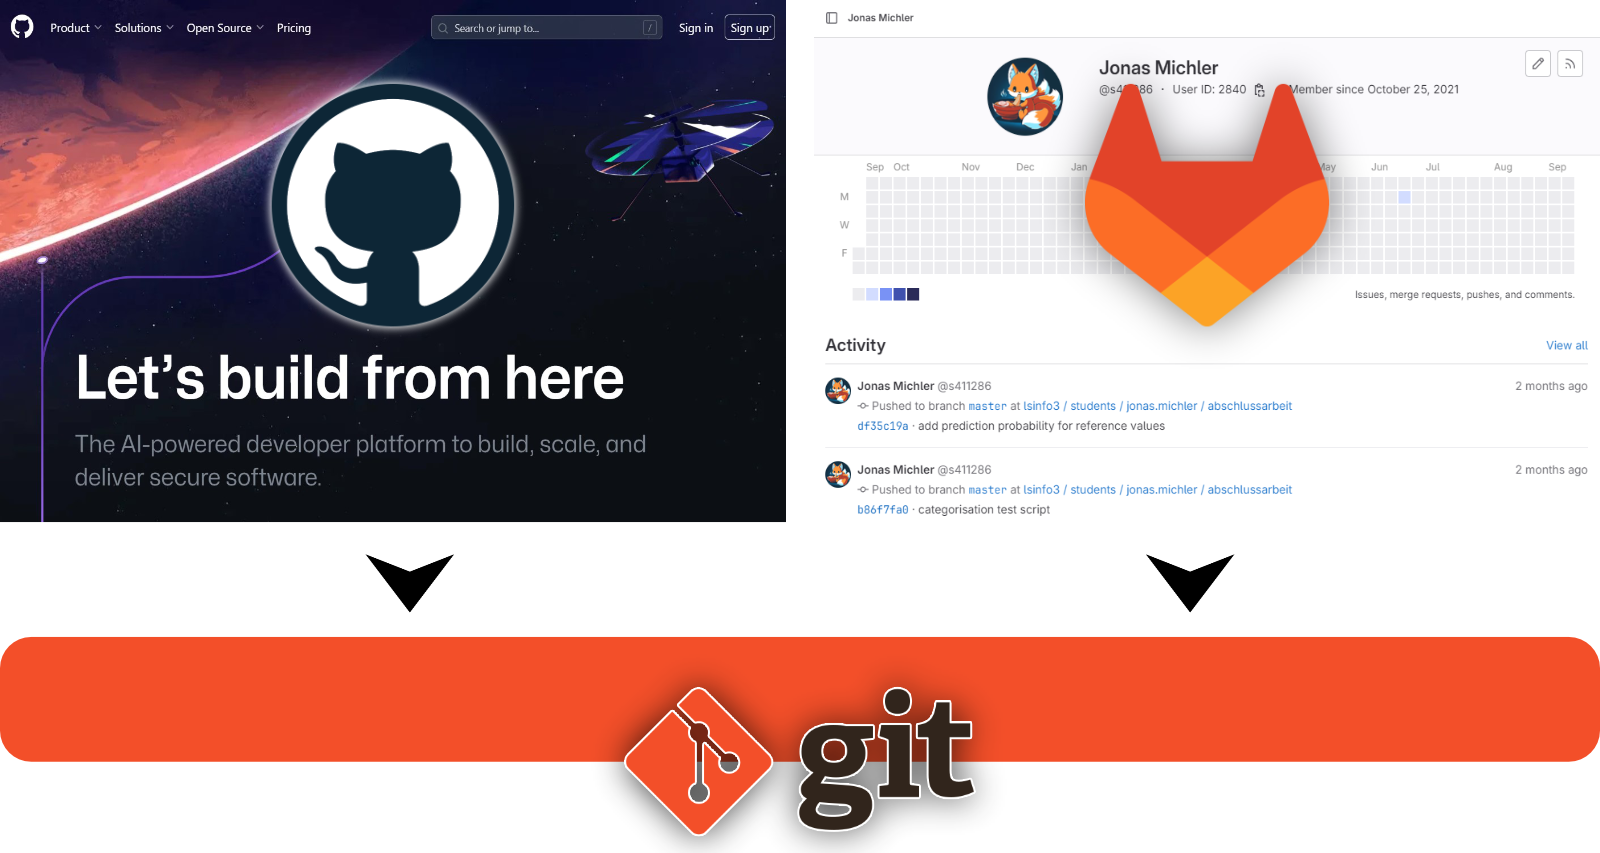
\includegraphics[width=0.7\textwidth]{assets/git-base.png}
		\end{figure}
	\end{frame}

	\begin{frame}{Vorteile von GitHub und GitLab}
		\begin{itemize}
			\item Versionsverwaltung von Code
			\begin{itemize}
				\item Effiziente Verwaltung und Nachverfolgung von Codeänderungen
				\item Historie zur Wiederherstellung früherer Versionen
			\end{itemize}
			\item Kollaborative Softwareentwicklung
			\begin{itemize}
				\item Gleichzeitige Zusammenarbeit mehrerer Entwickler
				\item Effektive Zusammenarbeit in dezentralen Teams
			\end{itemize}
			\item Unterstützung von Open Source und Privaten Projekten
			\begin{itemize}
				\item Plattformen ermöglichen öffentliche und private Repositories
				\item Schutz des geistigen Eigentums in privaten Projekten
			\end{itemize}
		\end{itemize}
	\end{frame}

	\begin{frame}{Cloud-basierte Versionskontrolle}
		\begin{figure}
			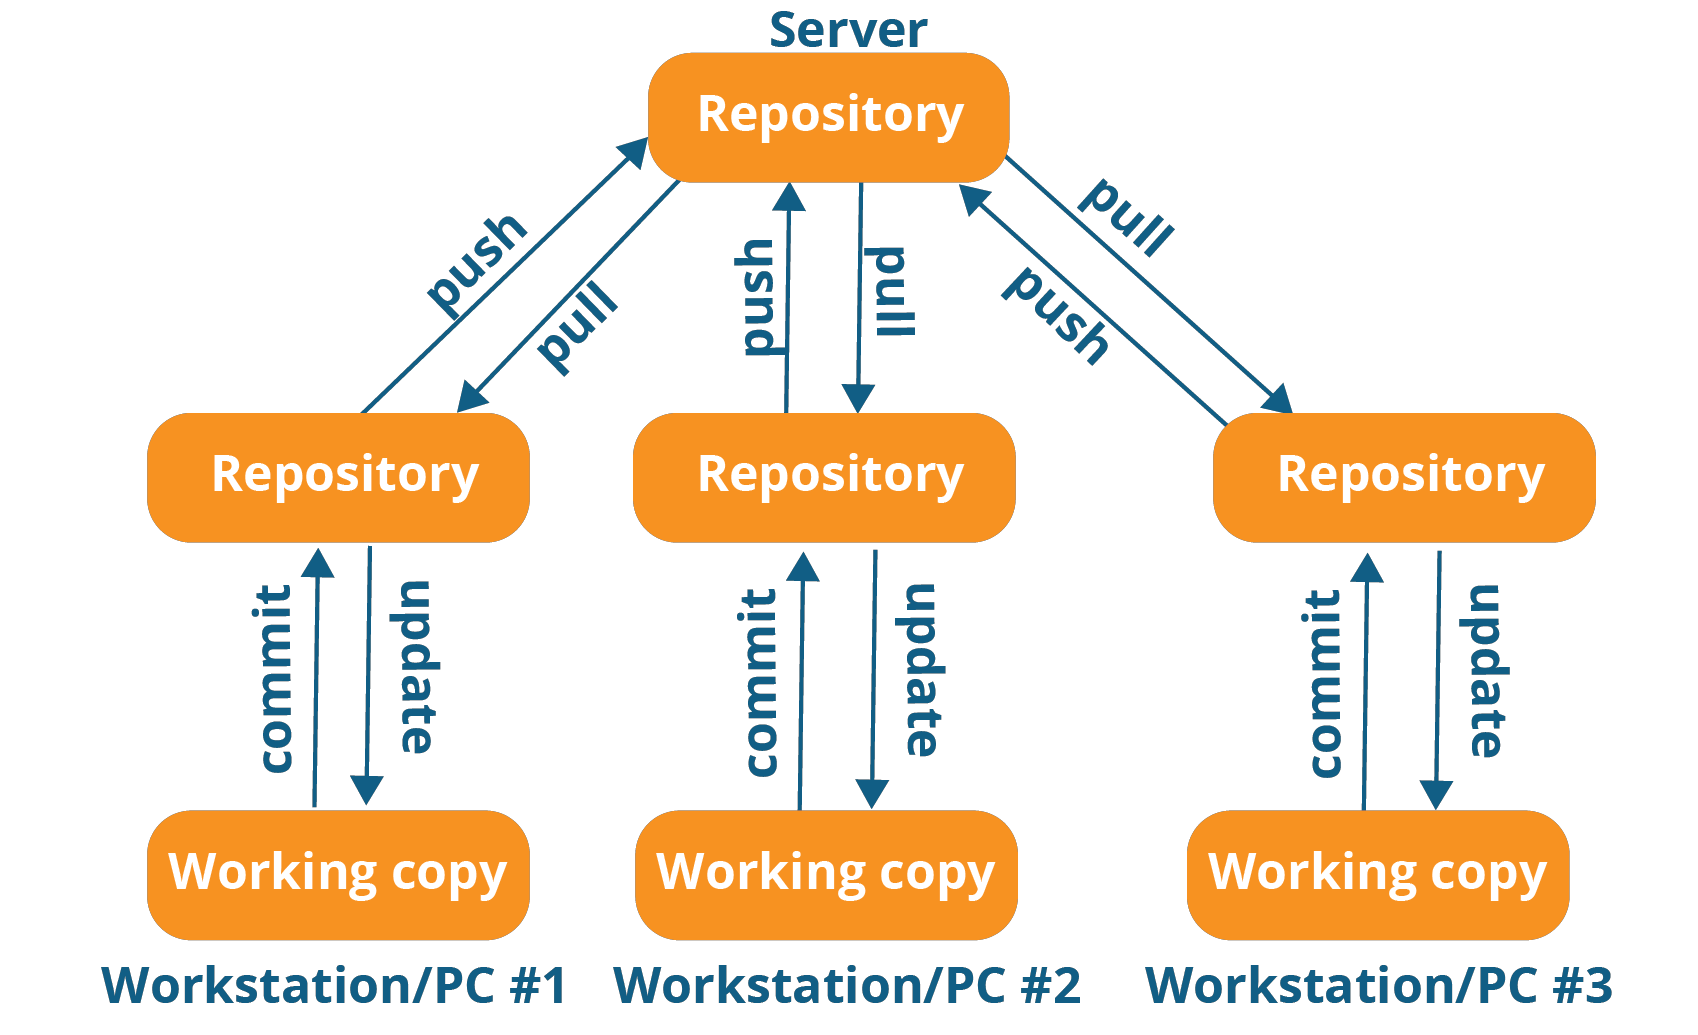
\includegraphics[width=0.6\textwidth]{assets/version-control.png}
			\caption{Distributed Version Control}
		\end{figure}
	\end{frame}
	
	\begin{frame}{Cloud-basierte Versionskontrolle}
		\begin{columns}
			\begin{column}{0.6\textwidth}
				\begin{itemize}
						\item Lokales Arbeitsrepository
						\item Änderungen können hochgeladen (gepusht) werden
						\item Änderungen von Teammitgliedern können aus der Cloud heruntergeladen werden
						\item Konflikte können auftreten, wenn mehrere Personen gleichzeitig arbeiten
				\end{itemize}
			\end{column}
			\begin{column}{0.4\textwidth}
				\begin{center}
					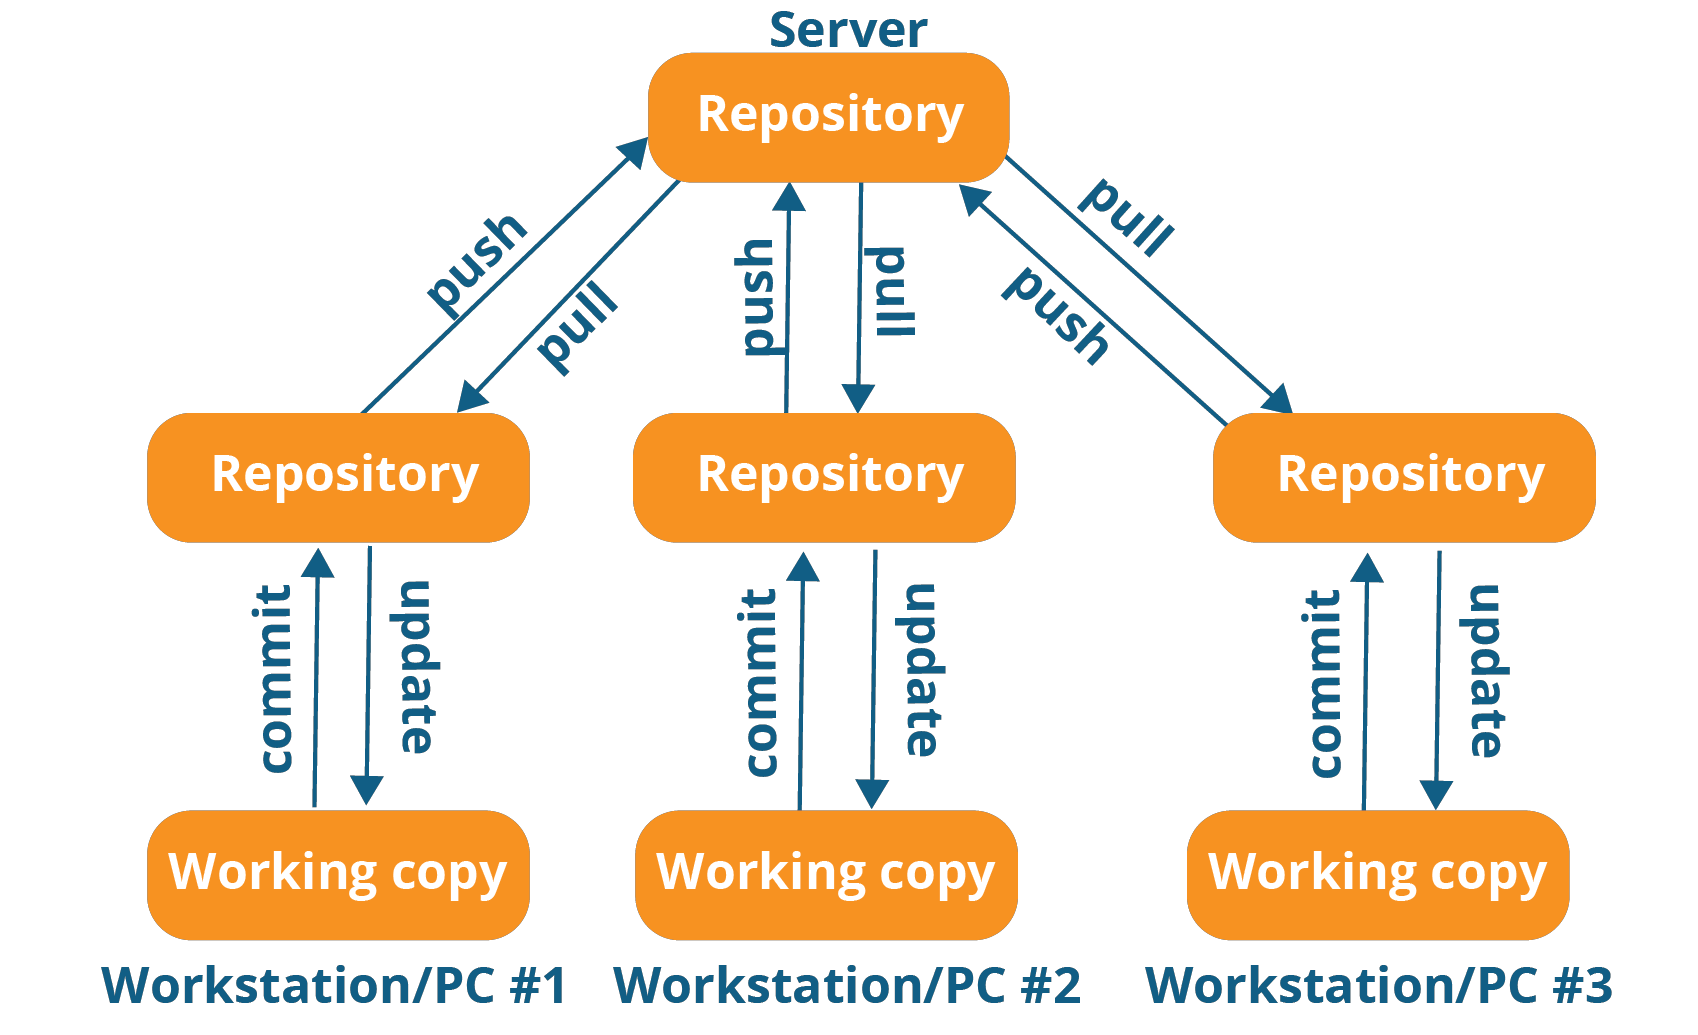
\includegraphics[width=0.9\textwidth]{assets/version-control.png}
					% Fügen Sie hier ein Bild ein, um die Idee der Cloud-Versionkontrolle zu veranschaulichen.
				\end{center}
			\end{column}
		\end{columns}
	\end{frame}
	
	\begin{frame}{GitHub vs. GitLab}
		\textbf{GitHub}
		\begin{itemize}
			\item Beliebte Plattform für Versionsverwaltung
			\item Hauptsächlich für Open Source-Projekte
			\item Funktionen: Issues, Pull Requests, Actions
			\item Cloud-basiert
		\end{itemize}
		\vspace{1em}
		\textbf{GitLab}
		\begin{itemize}
			\item Alternative mit ähnlichen Funktionen
			\item Geeignet für Open Source und private Projekte
			\item Umfassende CI/CD-Integration
			\item Cloud und lokale Installation
		\end{itemize}
	\end{frame}			
		
	\begin{frame}{GitHub vs. GitLab}
		\textbf{Hauptunterschiede:}
		\vspace{1em}
		\begin{columns}
			\begin{column}{0.5\textwidth}
				GitHub
				\begin{itemize}
					\item Nur Cloud
					\item Unternehmens- und OS-Lösungen
					\item Selbst nicht Open Source
					\item vielseitiges Ökosystem \(Copilot, Workspaces \dots\)
				\end{itemize}
			\end{column}
			\begin{column}{0.5\textwidth}
				GitLab
				\begin{itemize}
					\item Cloud und On-Premises
					\item Unternehmensorientierte Lösung
					\item komplett Open Source
					\item reine Git-Lösung
				\end{itemize}
			\end{column}
		\end{columns}
	\end{frame}
		

	\section{GitHub: Erste Schritte}
	
	\begin{frame}{GitHub}
		\begin{figure}
			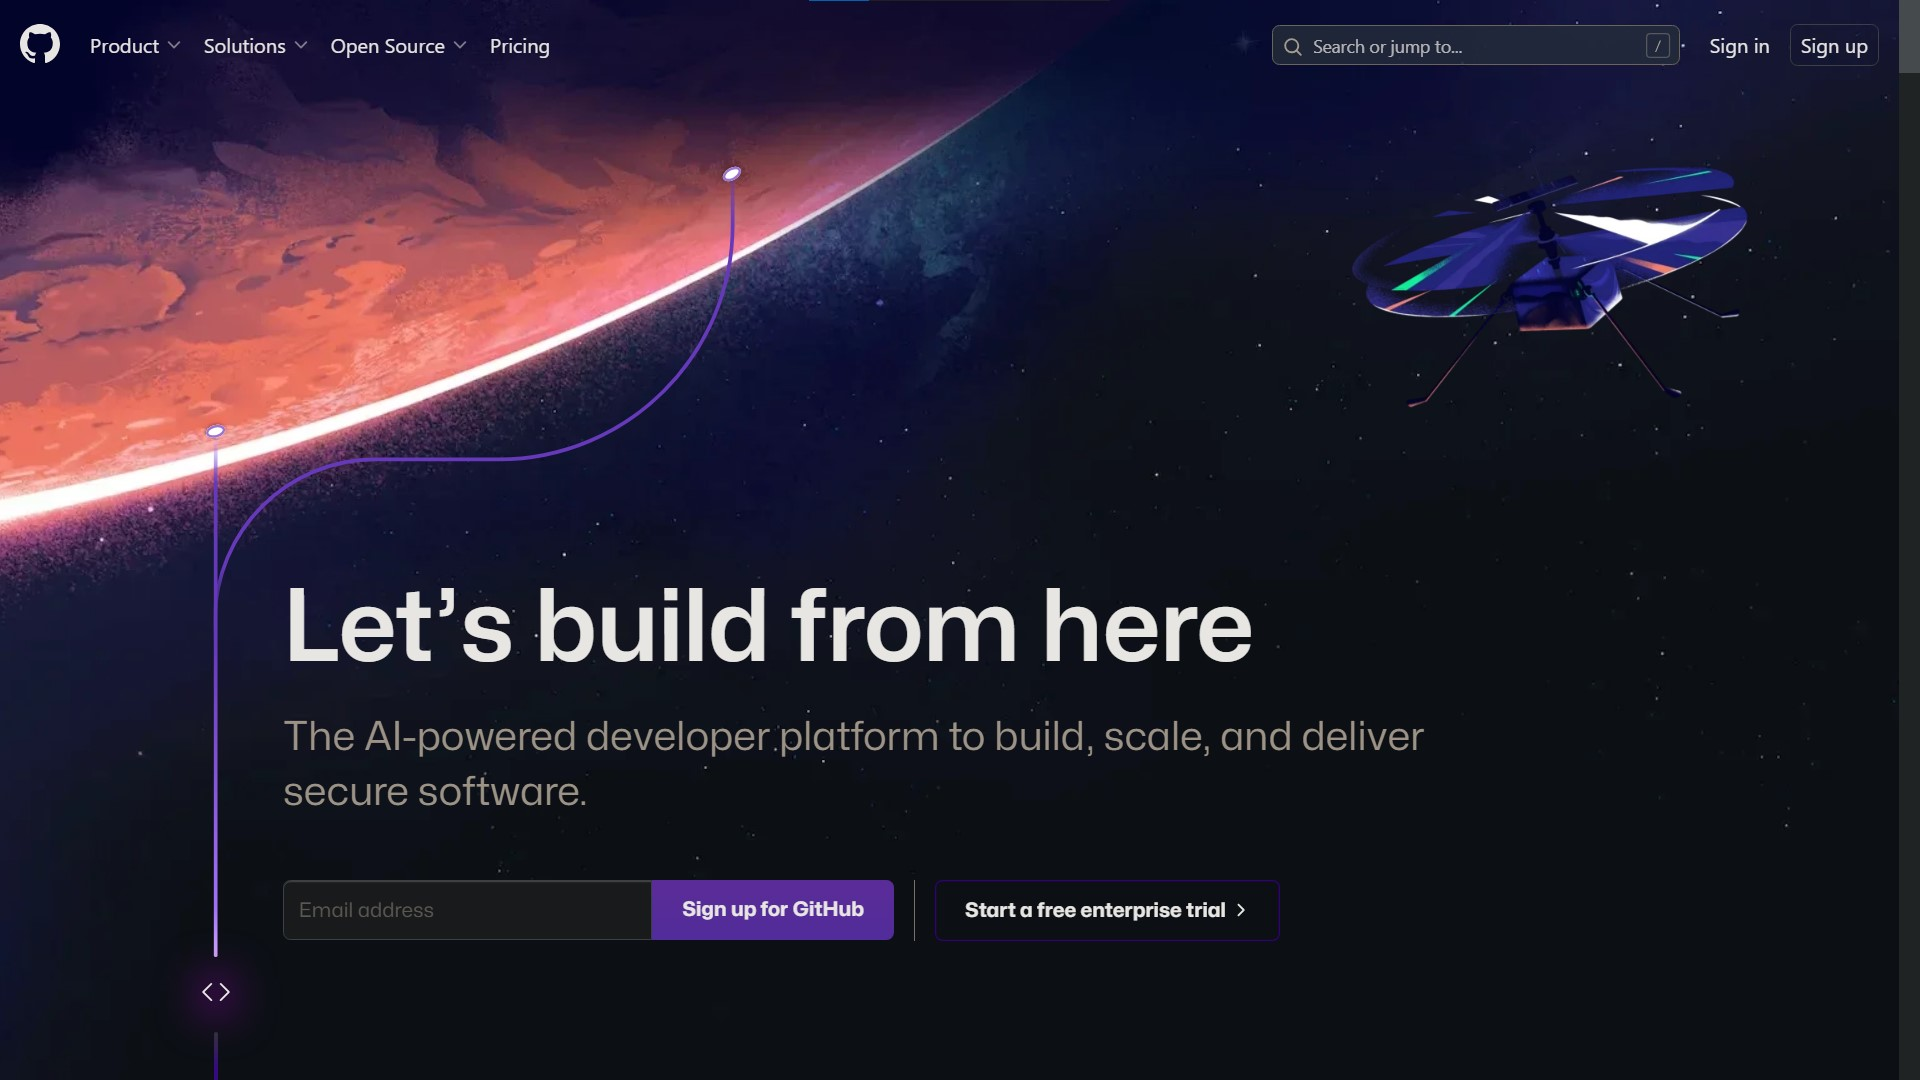
\includegraphics[width=0.6\textwidth]{assets/github/github-home.jpg}
			\caption{GitHub Homepage}
		\end{figure}
	\end{frame}

	\begin{frame}{GitHub: Anmeldung}
		\begin{columns}
			\begin{column}{0.5\textwidth}
				\begin{enumerate}
					\item \url{https://github.com} besuchen
					\item Schaltfläche ``Sign Up''
					\item E-Mail-Adresse + sicheres Passwort
					\item Benutzernamen wählen
					\item E-Mail-Verifizierung
				\end{enumerate}
			\end{column}
			\begin{column}{0.5\textwidth}
				% GitHub: your profile
				
\includegraphics[width=\textwidth]{assets/we-can-do-it.png}
			\end{column}
		\end{columns}
	\end{frame}

	\begin{frame}{GitHub: Profil einrichten}
		\begin{columns}
			\begin{column}{0.6\textwidth}
				\begin{enumerate}
					\item Profil-Icon (oben rechts), im Dropdown ``Your profile''
					\item Profilbild und eine kurze Beschreibung hinzufügen
					\item Weitere Informationen hinzufügen
					\item Soziale Links oder Website verknüpfen
					\item Speichern
				\end{enumerate}
			\end{column}
			\begin{column}{0.35\textwidth}
				% GitHub: your profile
				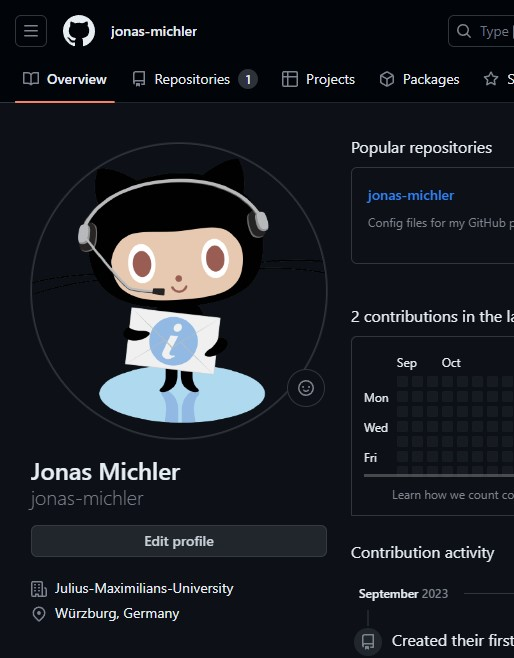
\includegraphics[width=\textwidth]{assets/github/your-profile.jpg}
			\end{column}
		\end{columns}
	\end{frame}


	\section{GitHub + GitLab}

	\begin{frame}{GitHub-Profil: Überblick}
		\textbf{Was Ihr GitHub-Profil zeigt:}
		\begin{itemize}
			\item Aktuelle Projekte
			\item Verwendete Programmiersprachen
			\item Ihre Follower und gefolgten Entwickler
		\end{itemize}
		\vspace{1em}
		\textbf{Warum ist es wichtig?}
		\begin{itemize}
			\item Arbeitgeber und Teams prüfen oft GitHub-Profile
			\item Zeigt Leidenschaft für Softwareentwicklung
			\item Dient als Portfolio Ihrer Fähigkeiten
			\item Ermöglicht Networking und Zusammenarbeit
		\end{itemize}
	\end{frame}

	\begin{frame}{Repository-Oberfläche}
		\begin{itemize}
			\item Code und Dateien im Repository
			\item README-Datei und Projektinformationen
			\item Contributors und Aktivitäten
			\item Branches und Pull Requests
			\item Projektstatistiken und Insights
		\end{itemize}
		Repos: 
		\begin{itemize}
			\item \url{https://github.com/facebook/react}
			\item \url{https://github.com/signalapp}
			\item \url{https://github.com/audacity/audacity}
		\end{itemize}
	\end{frame}


	% \section{GitLab}
	
	\begin{frame}{GitLab: Repository-Oberfläche}
		\begin{figure}
			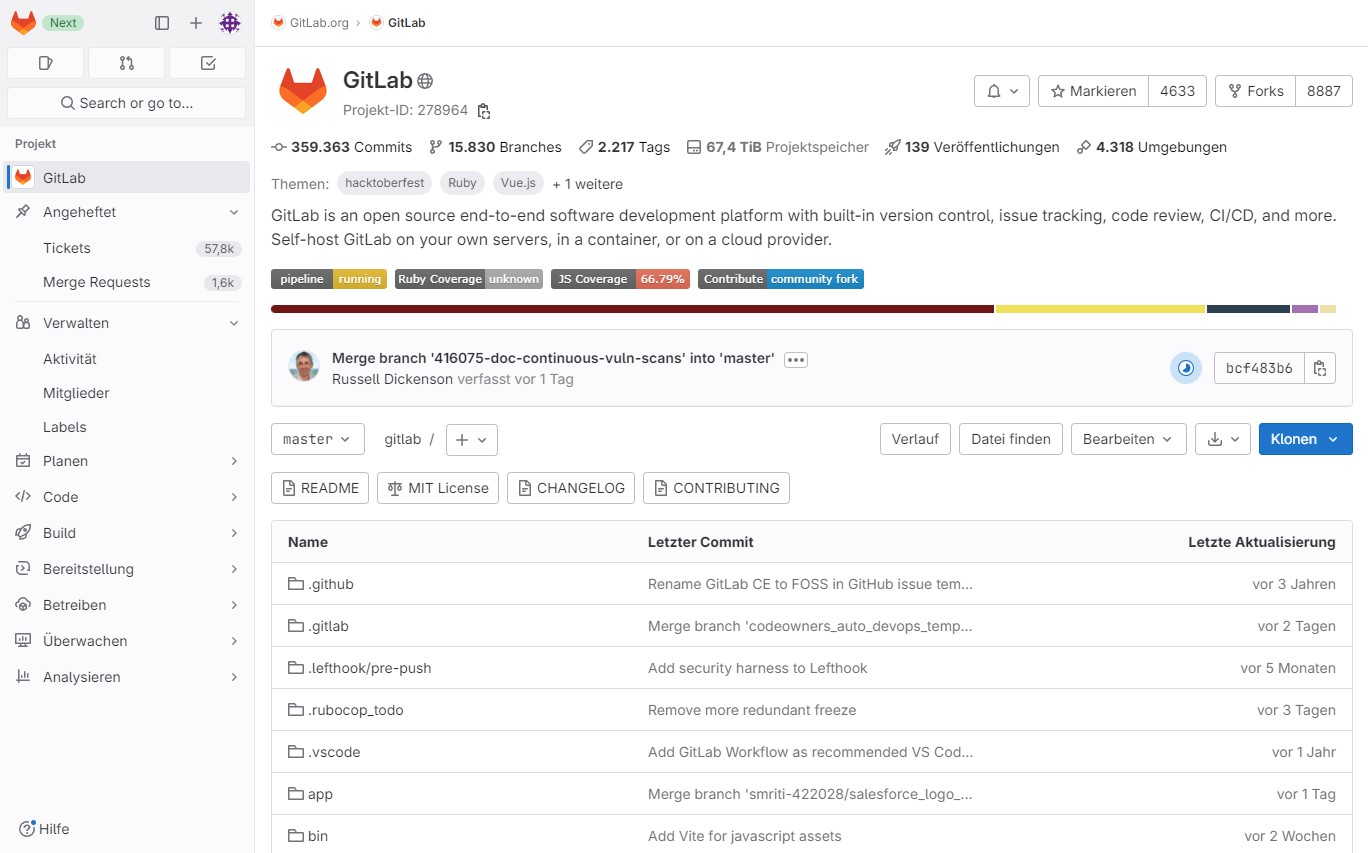
\includegraphics[width=0.6\textwidth]{assets/gitlab/repository.jpg}
			\caption{GitLab Repository}
		\end{figure}
		sample source: \url{https://gitlab.com/gitlab-org/gitlab}
	\end{frame}
	
	\begin{frame}{GitLab: Profil-Oberfläche}
		\begin{figure}
			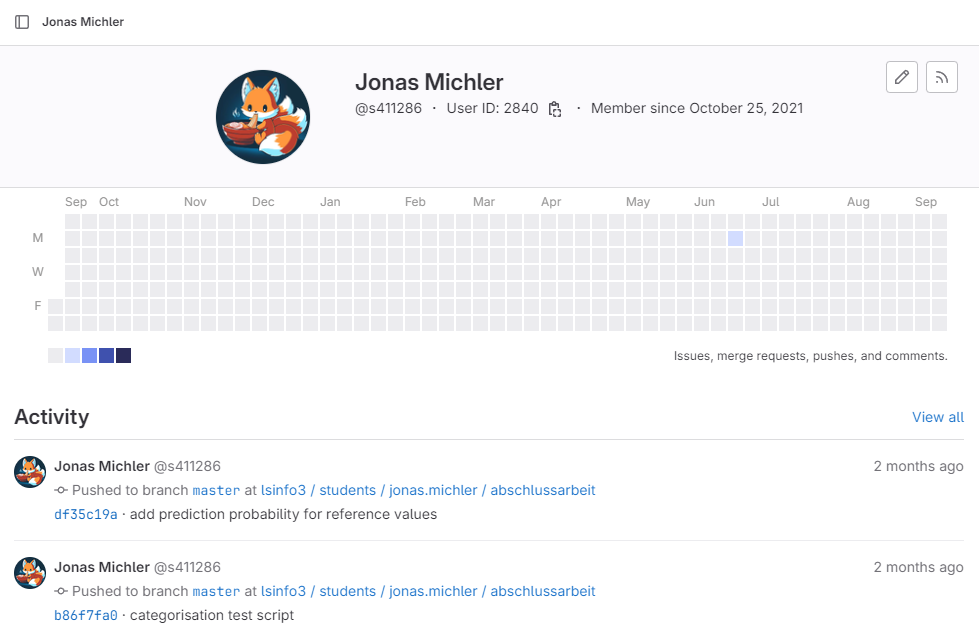
\includegraphics[width=0.6\textwidth]{assets/gitlab/profile.png}
			\caption{GitLab Profil}
		\end{figure}
	\end{frame}


	\section{Contribution}

	\begin{frame}{Contribution: Diverse Möglichkeiten zur Mitarbeit}
		\begin{itemize}
			\item \textbf{Code-Beitrag:}
				\begin{itemize}
					\item Schreiben neuer Funktionen
					\item Beheben von Fehlern
					\item Issues bearbeiten
				\end{itemize}
			\item \textbf{Fehlerberichte (Bug Reports):}
				\begin{itemize}
					\item Melden von Softwarefehlern oder Problemen
					\item Hilft bei der Fehlerbehebung und Verbesserung der Stabilität
				\end{itemize}
			\item \textbf{Dokumentation, Support und Diskussion:}
				\begin{itemize}
					\item Dokumentation/Wiki/FAQ ausarbeiten
					\item Beantworten von Fragen anderer Benutzer
					\item Teilnahme an Diskussionen und Entscheidungsfindung
				\end{itemize}
		\end{itemize}
	\end{frame}

	\begin{frame}{Erstellen detaillierter Fehlerbeschreibungen/Issues}
		\begin{itemize}
			\item Issues sind der Schlüssel zur Verfolgung von Fehlern und Verbesserungen
			\item Beschreiben Sie Fehler so detailliert wie möglich:
			\begin{itemize}
				\item Was ist das fehlerhafte Verhalten?
				\item Welche Schritte führen zum Fehler?
				\item Was ist das zu erwartende Verhalten?
				\item Welche Umgebung verwenden Sie?
				\item -> Guidelines beachten
			\end{itemize}
			\item Klare Beschreibungen erleichtern das Verständnis und die Replizierbarkeit
			\vspace{2em}
			\item Issues sind \textbf{nicht} der Ort, um seine persönliche Meinung zum Podukt zu veröffentlichen
		\end{itemize}
	\end{frame}

	\begin{frame}{Code-Beiträge an spezifische Probleme/Issues binden}
		\begin{itemize}
			\item Beiträge, Forks und Pull Requests sollten immer zu einem spezifischen Problem gehören
			\item Diese Verknüpfung ermöglicht eine klare Zuordnung von Änderungen
			\item Verbessert die Tranzparenz und Zusammenarbeit innerhalb des Projekts
			\vspace{2em}
			\item Viele Projekte besitzen eine Dokumantation, wie Beiträge einzureichen sind
			\begin{itemize}
				\item z.T. extern gelöst
			\end{itemize}
			\vspace{2em}
			\item Contribution.md, CodeOfConduct.md, SPDX
		\end{itemize}
	\end{frame}
	
	\begin{frame}{Code-Beitrag auf GitHub/GitLab}
		\begin{itemize}
			\item \textbf{Schritt 1: Fork des Projekts}
				\begin{itemize}
					\item Erstellen einer Kopie des Repositorys auf Ihrem eigenen Konto
				\end{itemize}
			\item \textbf{Schritt 2: Code ändern}
				\begin{itemize}
					\item Bearbeiten des Codes in Ihrem Fork
				\end{itemize}
			\item \textbf{Schritt 3: Pull/Merge Request erstellen}
				\begin{itemize}
					\item Reichen Sie Ihre Änderungen als Pull Request (PR) beim Hauptprojekt ein
				\end{itemize}
			\item \textbf{Schritt 4: Review Phase}
				\begin{itemize}
					\item Andere Entwickler überprüfen und diskutieren Ihre Änderungen.
				\end{itemize}
			\item \textbf{Schritt 5: Merge}
				\begin{itemize}
					\item Wenn Ihre Änderungen genehmigt werden, werden sie in das Hauptprojekt integriert
				\end{itemize}
		\end{itemize}
	\end{frame}	
	

	\begin{frame}{Repository erstellen}
		\begin{enumerate}
			\item Klicken Sie auf die Schaltfläche ``New'' oder ``+''
			\item Geben Sie einen Projektnamen und eine Beschreibung ein
			\item Legen Sie die Sichtbarkeit (öffentlich oder privat) fest
			\item Fügen Sie eine README-Datei hinzu, um Informationen über Ihr Projekt bereitzustellen
			\item Fügen Sie Ihrem Projekt eine Lizens bei
		\end{enumerate}
	\end{frame}


	\section{Zusammenfassung}

	\begin{frame}{GitHub + GitLab: Ihre Plattformen für kollaborative Entwicklung}
		\label{pg:lastpage} % Label on last frame to get the page number for footer
		\begin{columns}
			\begin{column}{0.4\textwidth}
				
\includegraphics[width=\textwidth]{assets/manufacturetocat.png}
			\end{column}
			\begin{column}{0.6\textwidth}
				\textbf{Warum GitHub und GitLab nutzen?}
				\begin{itemize}
					\item Gemeinschaftliche Arbeit an einem Projekt
					\item Dokumentation von Entwicklungsschritten
					\item Öffentliche Bereitstellung des Source-Code
					\item Möglichkeit spezifisches Feedback zu erhalten
				\end{itemize}
			\end{column}
		\end{columns}
	\end{frame}

	% \begin{frame}{References}
	% 	% References slide in appendix
	% 	\renewcommand*{\bibfont}{\normalfont\scriptsize}
	% 	\printbibliography[heading=none]
	% \end{frame}

\end{document}